\documentclass{article}
\usepackage{iclr2027_conference,times}
%%%%% NEW MATH DEFINITIONS %%%%%

\usepackage{amsmath,amsfonts,bm}

% Mark sections of captions for referring to divisions of figures
\newcommand{\figleft}{{\em (Left)}}
\newcommand{\figcenter}{{\em (Center)}}
\newcommand{\figright}{{\em (Right)}}
\newcommand{\figtop}{{\em (Top)}}
\newcommand{\figbottom}{{\em (Bottom)}}
\newcommand{\captiona}{{\em (a)}}
\newcommand{\captionb}{{\em (b)}}
\newcommand{\captionc}{{\em (c)}}
\newcommand{\captiond}{{\em (d)}}

% Highlight a newly defined term
\newcommand{\newterm}[1]{{\bf #1}}


% Figure reference, lower-case.
\def\figref#1{figure~\ref{#1}}
% Figure reference, capital. For start of sentence
\def\Figref#1{Figure~\ref{#1}}
\def\twofigref#1#2{figures \ref{#1} and \ref{#2}}
\def\quadfigref#1#2#3#4{figures \ref{#1}, \ref{#2}, \ref{#3} and \ref{#4}}
% Section reference, lower-case.
\def\secref#1{section~\ref{#1}}
% Section reference, capital.
\def\Secref#1{Section~\ref{#1}}
% Reference to two sections.
\def\twosecrefs#1#2{sections \ref{#1} and \ref{#2}}
% Reference to three sections.
\def\secrefs#1#2#3{sections \ref{#1}, \ref{#2} and \ref{#3}}
% Reference to an equation, lower-case.
\def\eqref#1{equation~\ref{#1}}
% Reference to an equation, upper case
\def\Eqref#1{Equation~\ref{#1}}
% A raw reference to an equation---avoid using if possible
\def\plaineqref#1{\ref{#1}}
% Reference to a chapter, lower-case.
\def\chapref#1{chapter~\ref{#1}}
% Reference to an equation, upper case.
\def\Chapref#1{Chapter~\ref{#1}}
% Reference to a range of chapters
\def\rangechapref#1#2{chapters\ref{#1}--\ref{#2}}
% Reference to an algorithm, lower-case.
\def\algref#1{algorithm~\ref{#1}}
% Reference to an algorithm, upper case.
\def\Algref#1{Algorithm~\ref{#1}}
\def\twoalgref#1#2{algorithms \ref{#1} and \ref{#2}}
\def\Twoalgref#1#2{Algorithms \ref{#1} and \ref{#2}}
% Reference to a part, lower case
\def\partref#1{part~\ref{#1}}
% Reference to a part, upper case
\def\Partref#1{Part~\ref{#1}}
\def\twopartref#1#2{parts \ref{#1} and \ref{#2}}

\def\ceil#1{\lceil #1 \rceil}
\def\floor#1{\lfloor #1 \rfloor}
\def\1{\bm{1}}
\newcommand{\train}{\mathcal{D}}
\newcommand{\valid}{\mathcal{D_{\mathrm{valid}}}}
\newcommand{\test}{\mathcal{D_{\mathrm{test}}}}

\def\eps{{\epsilon}}


% Random variables
\def\reta{{\textnormal{$\eta$}}}
\def\ra{{\textnormal{a}}}
\def\rb{{\textnormal{b}}}
\def\rc{{\textnormal{c}}}
\def\rd{{\textnormal{d}}}
\def\re{{\textnormal{e}}}
\def\rf{{\textnormal{f}}}
\def\rg{{\textnormal{g}}}
\def\rh{{\textnormal{h}}}
\def\ri{{\textnormal{i}}}
\def\rj{{\textnormal{j}}}
\def\rk{{\textnormal{k}}}
\def\rl{{\textnormal{l}}}
% rm is already a command, just don't name any random variables m
\def\rn{{\textnormal{n}}}
\def\ro{{\textnormal{o}}}
\def\rp{{\textnormal{p}}}
\def\rq{{\textnormal{q}}}
\def\rr{{\textnormal{r}}}
\def\rs{{\textnormal{s}}}
\def\rt{{\textnormal{t}}}
\def\ru{{\textnormal{u}}}
\def\rv{{\textnormal{v}}}
\def\rw{{\textnormal{w}}}
\def\rx{{\textnormal{x}}}
\def\ry{{\textnormal{y}}}
\def\rz{{\textnormal{z}}}

% Random vectors
\def\rvepsilon{{\mathbf{\epsilon}}}
\def\rvtheta{{\mathbf{\theta}}}
\def\rva{{\mathbf{a}}}
\def\rvb{{\mathbf{b}}}
\def\rvc{{\mathbf{c}}}
\def\rvd{{\mathbf{d}}}
\def\rve{{\mathbf{e}}}
\def\rvf{{\mathbf{f}}}
\def\rvg{{\mathbf{g}}}
\def\rvh{{\mathbf{h}}}
\def\rvu{{\mathbf{i}}}
\def\rvj{{\mathbf{j}}}
\def\rvk{{\mathbf{k}}}
\def\rvl{{\mathbf{l}}}
\def\rvm{{\mathbf{m}}}
\def\rvn{{\mathbf{n}}}
\def\rvo{{\mathbf{o}}}
\def\rvp{{\mathbf{p}}}
\def\rvq{{\mathbf{q}}}
\def\rvr{{\mathbf{r}}}
\def\rvs{{\mathbf{s}}}
\def\rvt{{\mathbf{t}}}
\def\rvu{{\mathbf{u}}}
\def\rvv{{\mathbf{v}}}
\def\rvw{{\mathbf{w}}}
\def\rvx{{\mathbf{x}}}
\def\rvy{{\mathbf{y}}}
\def\rvz{{\mathbf{z}}}

% Elements of random vectors
\def\erva{{\textnormal{a}}}
\def\ervb{{\textnormal{b}}}
\def\ervc{{\textnormal{c}}}
\def\ervd{{\textnormal{d}}}
\def\erve{{\textnormal{e}}}
\def\ervf{{\textnormal{f}}}
\def\ervg{{\textnormal{g}}}
\def\ervh{{\textnormal{h}}}
\def\ervi{{\textnormal{i}}}
\def\ervj{{\textnormal{j}}}
\def\ervk{{\textnormal{k}}}
\def\ervl{{\textnormal{l}}}
\def\ervm{{\textnormal{m}}}
\def\ervn{{\textnormal{n}}}
\def\ervo{{\textnormal{o}}}
\def\ervp{{\textnormal{p}}}
\def\ervq{{\textnormal{q}}}
\def\ervr{{\textnormal{r}}}
\def\ervs{{\textnormal{s}}}
\def\ervt{{\textnormal{t}}}
\def\ervu{{\textnormal{u}}}
\def\ervv{{\textnormal{v}}}
\def\ervw{{\textnormal{w}}}
\def\ervx{{\textnormal{x}}}
\def\ervy{{\textnormal{y}}}
\def\ervz{{\textnormal{z}}}

% Random matrices
\def\rmA{{\mathbf{A}}}
\def\rmB{{\mathbf{B}}}
\def\rmC{{\mathbf{C}}}
\def\rmD{{\mathbf{D}}}
\def\rmE{{\mathbf{E}}}
\def\rmF{{\mathbf{F}}}
\def\rmG{{\mathbf{G}}}
\def\rmH{{\mathbf{H}}}
\def\rmI{{\mathbf{I}}}
\def\rmJ{{\mathbf{J}}}
\def\rmK{{\mathbf{K}}}
\def\rmL{{\mathbf{L}}}
\def\rmM{{\mathbf{M}}}
\def\rmN{{\mathbf{N}}}
\def\rmO{{\mathbf{O}}}
\def\rmP{{\mathbf{P}}}
\def\rmQ{{\mathbf{Q}}}
\def\rmR{{\mathbf{R}}}
\def\rmS{{\mathbf{S}}}
\def\rmT{{\mathbf{T}}}
\def\rmU{{\mathbf{U}}}
\def\rmV{{\mathbf{V}}}
\def\rmW{{\mathbf{W}}}
\def\rmX{{\mathbf{X}}}
\def\rmY{{\mathbf{Y}}}
\def\rmZ{{\mathbf{Z}}}

% Elements of random matrices
\def\ermA{{\textnormal{A}}}
\def\ermB{{\textnormal{B}}}
\def\ermC{{\textnormal{C}}}
\def\ermD{{\textnormal{D}}}
\def\ermE{{\textnormal{E}}}
\def\ermF{{\textnormal{F}}}
\def\ermG{{\textnormal{G}}}
\def\ermH{{\textnormal{H}}}
\def\ermI{{\textnormal{I}}}
\def\ermJ{{\textnormal{J}}}
\def\ermK{{\textnormal{K}}}
\def\ermL{{\textnormal{L}}}
\def\ermM{{\textnormal{M}}}
\def\ermN{{\textnormal{N}}}
\def\ermO{{\textnormal{O}}}
\def\ermP{{\textnormal{P}}}
\def\ermQ{{\textnormal{Q}}}
\def\ermR{{\textnormal{R}}}
\def\ermS{{\textnormal{S}}}
\def\ermT{{\textnormal{T}}}
\def\ermU{{\textnormal{U}}}
\def\ermV{{\textnormal{V}}}
\def\ermW{{\textnormal{W}}}
\def\ermX{{\textnormal{X}}}
\def\ermY{{\textnormal{Y}}}
\def\ermZ{{\textnormal{Z}}}

% Vectors
\def\vzero{{\bm{0}}}
\def\vone{{\bm{1}}}
\def\vmu{{\bm{\mu}}}
\def\vtheta{{\bm{\theta}}}
\def\va{{\bm{a}}}
\def\vb{{\bm{b}}}
\def\vc{{\bm{c}}}
\def\vd{{\bm{d}}}
\def\ve{{\bm{e}}}
\def\vf{{\bm{f}}}
\def\vg{{\bm{g}}}
\def\vh{{\bm{h}}}
\def\vi{{\bm{i}}}
\def\vj{{\bm{j}}}
\def\vk{{\bm{k}}}
\def\vl{{\bm{l}}}
\def\vm{{\bm{m}}}
\def\vn{{\bm{n}}}
\def\vo{{\bm{o}}}
\def\vp{{\bm{p}}}
\def\vq{{\bm{q}}}
\def\vr{{\bm{r}}}
\def\vs{{\bm{s}}}
\def\vt{{\bm{t}}}
\def\vu{{\bm{u}}}
\def\vv{{\bm{v}}}
\def\vw{{\bm{w}}}
\def\vx{{\bm{x}}}
\def\vy{{\bm{y}}}
\def\vz{{\bm{z}}}

% Elements of vectors
\def\evalpha{{\alpha}}
\def\evbeta{{\beta}}
\def\evepsilon{{\epsilon}}
\def\evlambda{{\lambda}}
\def\evomega{{\omega}}
\def\evmu{{\mu}}
\def\evpsi{{\psi}}
\def\evsigma{{\sigma}}
\def\evtheta{{\theta}}
\def\eva{{a}}
\def\evb{{b}}
\def\evc{{c}}
\def\evd{{d}}
\def\eve{{e}}
\def\evf{{f}}
\def\evg{{g}}
\def\evh{{h}}
\def\evi{{i}}
\def\evj{{j}}
\def\evk{{k}}
\def\evl{{l}}
\def\evm{{m}}
\def\evn{{n}}
\def\evo{{o}}
\def\evp{{p}}
\def\evq{{q}}
\def\evr{{r}}
\def\evs{{s}}
\def\evt{{t}}
\def\evu{{u}}
\def\evv{{v}}
\def\evw{{w}}
\def\evx{{x}}
\def\evy{{y}}
\def\evz{{z}}

% Matrix
\def\mA{{\bm{A}}}
\def\mB{{\bm{B}}}
\def\mC{{\bm{C}}}
\def\mD{{\bm{D}}}
\def\mE{{\bm{E}}}
\def\mF{{\bm{F}}}
\def\mG{{\bm{G}}}
\def\mH{{\bm{H}}}
\def\mI{{\bm{I}}}
\def\mJ{{\bm{J}}}
\def\mK{{\bm{K}}}
\def\mL{{\bm{L}}}
\def\mM{{\bm{M}}}
\def\mN{{\bm{N}}}
\def\mO{{\bm{O}}}
\def\mP{{\bm{P}}}
\def\mQ{{\bm{Q}}}
\def\mR{{\bm{R}}}
\def\mS{{\bm{S}}}
\def\mT{{\bm{T}}}
\def\mU{{\bm{U}}}
\def\mV{{\bm{V}}}
\def\mW{{\bm{W}}}
\def\mX{{\bm{X}}}
\def\mY{{\bm{Y}}}
\def\mZ{{\bm{Z}}}
\def\mBeta{{\bm{\beta}}}
\def\mPhi{{\bm{\Phi}}}
\def\mLambda{{\bm{\Lambda}}}
\def\mSigma{{\bm{\Sigma}}}

% Tensor
\DeclareMathAlphabet{\mathsfit}{\encodingdefault}{\sfdefault}{m}{sl}
\SetMathAlphabet{\mathsfit}{bold}{\encodingdefault}{\sfdefault}{bx}{n}
\newcommand{\tens}[1]{\bm{\mathsfit{#1}}}
\def\tA{{\tens{A}}}
\def\tB{{\tens{B}}}
\def\tC{{\tens{C}}}
\def\tD{{\tens{D}}}
\def\tE{{\tens{E}}}
\def\tF{{\tens{F}}}
\def\tG{{\tens{G}}}
\def\tH{{\tens{H}}}
\def\tI{{\tens{I}}}
\def\tJ{{\tens{J}}}
\def\tK{{\tens{K}}}
\def\tL{{\tens{L}}}
\def\tM{{\tens{M}}}
\def\tN{{\tens{N}}}
\def\tO{{\tens{O}}}
\def\tP{{\tens{P}}}
\def\tQ{{\tens{Q}}}
\def\tR{{\tens{R}}}
\def\tS{{\tens{S}}}
\def\tT{{\tens{T}}}
\def\tU{{\tens{U}}}
\def\tV{{\tens{V}}}
\def\tW{{\tens{W}}}
\def\tX{{\tens{X}}}
\def\tY{{\tens{Y}}}
\def\tZ{{\tens{Z}}}


% Graph
\def\gA{{\mathcal{A}}}
\def\gB{{\mathcal{B}}}
\def\gC{{\mathcal{C}}}
\def\gD{{\mathcal{D}}}
\def\gE{{\mathcal{E}}}
\def\gF{{\mathcal{F}}}
\def\gG{{\mathcal{G}}}
\def\gH{{\mathcal{H}}}
\def\gI{{\mathcal{I}}}
\def\gJ{{\mathcal{J}}}
\def\gK{{\mathcal{K}}}
\def\gL{{\mathcal{L}}}
\def\gM{{\mathcal{M}}}
\def\gN{{\mathcal{N}}}
\def\gO{{\mathcal{O}}}
\def\gP{{\mathcal{P}}}
\def\gQ{{\mathcal{Q}}}
\def\gR{{\mathcal{R}}}
\def\gS{{\mathcal{S}}}
\def\gT{{\mathcal{T}}}
\def\gU{{\mathcal{U}}}
\def\gV{{\mathcal{V}}}
\def\gW{{\mathcal{W}}}
\def\gX{{\mathcal{X}}}
\def\gY{{\mathcal{Y}}}
\def\gZ{{\mathcal{Z}}}

% Sets
\def\sA{{\mathbb{A}}}
\def\sB{{\mathbb{B}}}
\def\sC{{\mathbb{C}}}
\def\sD{{\mathbb{D}}}
% Don't use a set called E, because this would be the same as our symbol
% for expectation.
\def\sF{{\mathbb{F}}}
\def\sG{{\mathbb{G}}}
\def\sH{{\mathbb{H}}}
\def\sI{{\mathbb{I}}}
\def\sJ{{\mathbb{J}}}
\def\sK{{\mathbb{K}}}
\def\sL{{\mathbb{L}}}
\def\sM{{\mathbb{M}}}
\def\sN{{\mathbb{N}}}
\def\sO{{\mathbb{O}}}
\def\sP{{\mathbb{P}}}
\def\sQ{{\mathbb{Q}}}
\def\sR{{\mathbb{R}}}
\def\sS{{\mathbb{S}}}
\def\sT{{\mathbb{T}}}
\def\sU{{\mathbb{U}}}
\def\sV{{\mathbb{V}}}
\def\sW{{\mathbb{W}}}
\def\sX{{\mathbb{X}}}
\def\sY{{\mathbb{Y}}}
\def\sZ{{\mathbb{Z}}}

% Entries of a matrix
\def\emLambda{{\Lambda}}
\def\emA{{A}}
\def\emB{{B}}
\def\emC{{C}}
\def\emD{{D}}
\def\emE{{E}}
\def\emF{{F}}
\def\emG{{G}}
\def\emH{{H}}
\def\emI{{I}}
\def\emJ{{J}}
\def\emK{{K}}
\def\emL{{L}}
\def\emM{{M}}
\def\emN{{N}}
\def\emO{{O}}
\def\emP{{P}}
\def\emQ{{Q}}
\def\emR{{R}}
\def\emS{{S}}
\def\emT{{T}}
\def\emU{{U}}
\def\emV{{V}}
\def\emW{{W}}
\def\emX{{X}}
\def\emY{{Y}}
\def\emZ{{Z}}
\def\emSigma{{\Sigma}}

% entries of a tensor
% Same font as tensor, without \bm wrapper
\newcommand{\etens}[1]{\mathsfit{#1}}
\def\etLambda{{\etens{\Lambda}}}
\def\etA{{\etens{A}}}
\def\etB{{\etens{B}}}
\def\etC{{\etens{C}}}
\def\etD{{\etens{D}}}
\def\etE{{\etens{E}}}
\def\etF{{\etens{F}}}
\def\etG{{\etens{G}}}
\def\etH{{\etens{H}}}
\def\etI{{\etens{I}}}
\def\etJ{{\etens{J}}}
\def\etK{{\etens{K}}}
\def\etL{{\etens{L}}}
\def\etM{{\etens{M}}}
\def\etN{{\etens{N}}}
\def\etO{{\etens{O}}}
\def\etP{{\etens{P}}}
\def\etQ{{\etens{Q}}}
\def\etR{{\etens{R}}}
\def\etS{{\etens{S}}}
\def\etT{{\etens{T}}}
\def\etU{{\etens{U}}}
\def\etV{{\etens{V}}}
\def\etW{{\etens{W}}}
\def\etX{{\etens{X}}}
\def\etY{{\etens{Y}}}
\def\etZ{{\etens{Z}}}

% The true underlying data generating distribution
\newcommand{\pdata}{p_{\rm{data}}}
% The empirical distribution defined by the training set
\newcommand{\ptrain}{\hat{p}_{\rm{data}}}
\newcommand{\Ptrain}{\hat{P}_{\rm{data}}}
% The model distribution
\newcommand{\pmodel}{p_{\rm{model}}}
\newcommand{\Pmodel}{P_{\rm{model}}}
\newcommand{\ptildemodel}{\tilde{p}_{\rm{model}}}
% Stochastic autoencoder distributions
\newcommand{\pencode}{p_{\rm{encoder}}}
\newcommand{\pdecode}{p_{\rm{decoder}}}
\newcommand{\precons}{p_{\rm{reconstruct}}}

\newcommand{\laplace}{\mathrm{Laplace}} % Laplace distribution

\newcommand{\E}{\mathbb{E}}
\newcommand{\Ls}{\mathcal{L}}
\newcommand{\R}{\mathbb{R}}
\newcommand{\emp}{\tilde{p}}
\newcommand{\lr}{\alpha}
\newcommand{\reg}{\lambda}
\newcommand{\rect}{\mathrm{rectifier}}
\newcommand{\softmax}{\mathrm{softmax}}
\newcommand{\sigmoid}{\sigma}
\newcommand{\softplus}{\zeta}
\newcommand{\KL}{D_{\mathrm{KL}}}
\newcommand{\Var}{\mathrm{Var}}
\newcommand{\standarderror}{\mathrm{SE}}
\newcommand{\Cov}{\mathrm{Cov}}
% Wolfram Mathworld says $L^2$ is for function spaces and $\ell^2$ is for vectors
% But then they seem to use $L^2$ for vectors throughout the site, and so does
% wikipedia.
\newcommand{\normlzero}{L^0}
\newcommand{\normlone}{L^1}
\newcommand{\normltwo}{L^2}
\newcommand{\normlp}{L^p}
\newcommand{\normmax}{L^\infty}

\newcommand{\parents}{Pa} % See usage in notation.tex. Chosen to match Daphne's book.

\DeclareMathOperator*{\argmax}{arg\,max}
\DeclareMathOperator*{\argmin}{arg\,min}

\DeclareMathOperator{\sign}{sign}
\DeclareMathOperator{\Tr}{Tr}
\let\ab\allowbreak

\usepackage{amsmath,amssymb,mathtools}
\usepackage{booktabs}
\usepackage{tabularx}
\usepackage{multirow}
\usepackage{graphicx}
\usepackage{placeins}
\usepackage{hyperref}
\usepackage{xcolor}
\usepackage{url}
\hypersetup{hidelinks}
\usepackage[normalem]{ulem}
\makeatletter
\DeclareRobustCommand{\del}[1]{{\color{red}%
  \let\del@cite\cite \let\del@citep\citep \let\del@citet\citet
  \let\del@ref\ref \let\del@eqref\eqref
  \renewcommand{\cite}[1]{\mbox{\del@cite{##1}}}%
  \renewcommand{\citep}[1]{\mbox{\del@citep{##1}}}%
  \renewcommand{\citet}[1]{\mbox{\del@citet{##1}}}%
  \renewcommand{\ref}[1]{\mbox{\del@ref{##1}}}%
  \renewcommand{\eqref}[1]{\mbox{\del@eqref{##1}}}%
  \sout{#1}}}
\makeatother
\newcommand{\add}[1]{{\color{blue}#1}}

\newcommand{\Hpre}{H^{\mathrm{pre}}}
\newcommand{\Hpost}{H^{\mathrm{post}}}
\newcommand{\Hres}{H^{\mathrm{res}}}
\newcommand{\norm}[1]{\lVert #1\rVert}

\title{ITO-HC: Identity-Centered Tanh Off-Diagonal Hyper-Connections}
% Keep the author block anonymous for submission.
\author{}

\begin{document}
\maketitle

\begin{abstract}
\add{[[Shi-Yuk: title should be left-adjusted, as per "iclr style reference.tex"]]}
Hyper-Connections (HC) widen the residual state and learn dynamic read, write, and stream-mixing maps. Manifold-Constrained Hyper-Connections (mHC) stabilize these maps by projecting the residual mixer onto the Birkhoff polytope. However, repeated positive mixing can contract stream-difference directions, while finite Sinkhorn iterations incur projection error. We propose \emph{ITO-HC}, which centers the residual mixer at the identity and adds a bounded, signed off-diagonal perturbation. This preserves an exact unit diagonal while retaining dynamic pre/post routers and nonlinear Transformer branches. We derive a layer-attention interpretation, characterize the rank-$n$ factorization induced by identity routing, and establish conditional stability bounds. In the available large-model runs, ITO-HC improves over identity-residual baseline (iHC) at every tested width from $n=4$ to $64$; at $n=64$ its validation loss is $3.0310$ versus $3.0606$ for identity. These results are single-run measurements, and the remaining comparison cells are reported explicitly as missing.
\end{abstract}

\section{Introduction}

Residual connections provide a short, well-conditioned identity path through depth \citep{he2016deep}. Hyper-Connections (HC) generalize this path by maintaining $n$ residual streams and learning how a branch reads from and writes to those streams \citep{zhu2024hyper}. A layer can be written as
\begin{equation}
 X_{l+1}=\Hres_l X_l+\Hpost_l f_l(\Hpre_l X_l;W_l),
 \label{eq:hc}
\end{equation}
where $X_l\in\R^{n\times C}$, $\Hpre_l\in\R^{1\times n}$, $\Hpost_l\in\R^{n\times 1}$, and $\Hres_l\in\R^{n\times n}$. The additional streams create paths for feature reuse across depth, but an unconstrained product of residual mixers can amplify, attenuate, or rotate the residual state. mHC addresses this issue by projecting dynamic residual matrices onto the Birkhoff polytope with Sinkhorn--Knopp iterations \citep{xie2026mhc}. mHC-lite replaces iterative projection with an exact convex-combination parameterization of permutation matrices \citep{yang2026mhclite}. KromHC uses a Kronecker parameterization to reduce the residual-matrix cost \citep{zhou2026kromhc}. More recently, Spectral-Sphere-Constrained Hyper-Connections (sHC) identify limitations of the Birkhoff constraint, including nonnegative convex mixing and parameterization inefficiency, and allow signed mixing under affine and spectral constraints \citep{liu2026shc}.
We use \emph{iHC} to denote the identity-residual baseline, namely the setting $\Hres_l=I$ at every layer while retaining the learned pre/post routers and the nonlinear branch. Thus iHC removes only residual-path mixing; it does not reduce the full Hyper-Connection block to an identity map.
\add{Shi-Yuk: mention iHC here. This is the main baseline but never get mentioned in the Introduction. Then you may replace occurence of \textit{identity routing} to iHC.}

\del{This work} \add{We} asks whether a fully learned residual mixer is necessary when the pre/post routers and the branch $f_l$ remain learned. We use the following bounded, identity-centered parameterization:
\begin{equation}
 \Hres_l=I+\gamma_l(\mathbf 1\mathbf 1^\top-I)\odot\tanh(S_l),
 \label{eq:method-short}
\end{equation}
where $S_l$ is a learned, possibly input-dependent logit matrix and $\gamma_l>0$ controls the maximum off-diagonal magnitude. We call this parameterization ITO-HC. It preserves the self highway, permits signed cross-stream corrections, and avoids a depth-long chain of strictly positive averages.

Our contributions are: \add{[[Shi-Yuk: May make this a full paragraph to save space?]]} we formulate ITO-HC and connect it to the layer-attention view of HC; characterize the rank-$n$ dense channel kernel induced by iHC while explaining why the causal mask and dynamic routers prevent it from fully characterizing network expressivity; give perturbation and spectral-norm conditions for the identity-centered residual path and compare its scaling with dynamic mHC and mHC-lite; and evaluate the method on OpenWebText with GPT-2-style models over $n\in\{4,8,16,32,64\}$.
\section{Background and Implementation}

\subsection{Related work}
HC broadens the residual pathway with multiple streams and learned read, write, and residual maps \citep{zhu2024hyper}. mHC constrains the residual mixer to the Birkhoff polytope of doubly stochastic matrices using Sinkhorn--Knopp projection \citep{xie2026mhc}; mHC-lite and KromHC replace this iterative projection with exact permutation-mixture and Kronecker parameterizations, respectively \citep{yang2026mhclite,zhou2026kromhc}. The iHC baseline fixes the residual mixer to $I$ while retaining learned pre/post routing. sHC argues that nonnegativity can limit signed feature interactions and that Birkhoff-constrained mixers may degenerate toward identity \citep{liu2026shc}. These methods motivate our identity-centered, signed off-diagonal parameterization; the detailed contraction comparison appears below.

\subsection{Multi-stream residual computation}
At layer $l$, the branch input and output are
\begin{equation}
 z_l=\Hpre_l X_l,\qquad y_l=f_l(z_l;W_l),\qquad
 X_{l+1}=\Hres_lX_l+\Hpost_l y_l.
 \label{eq:update}
\end{equation}
\del{In our implementation, each coefficient is the sum of a static logit and an input-dependent logit generated from the RMS-normalized, flattened stream state. }
For the generic HC/mHC parameterization, each read, write, and residual logit is the sum of a learned input-independent term and an input-dependent linear projection of the flattened, RMS-normalized stream state, scaled by a small learned gate \citep{zhu2024hyper,xie2026mhc}. In the main ITO-HC experiments, the pre/post routers retain this dynamic parameterization, whereas the residual correction is static: the dynamic residual generator is disabled and $S_l$ in Eq.~\ref{eq:full-method} is a learned layer-specific matrix. The iHC baseline uses the same pre/post routers with $\Hres_l=I$. This convention is distinct from the static/static and mixed static/dynamic ablations in Section~\ref{sec:dynamic-pre-post-ablation}.
Small learned gates scale the dynamic pre, residual, and post components whenever the corresponding dynamic generator is enabled. \del{The branch is an ordinary Transformer block: LayerNorm followed by causal self-attention, or LayerNorm followed by a two-layer GELU MLP.} 
\add{Each branch $f_l$ is one Transformer sublayer: LayerNorm followed by causal self-attention, or LayerNorm followed by a two-layer MLP with GELU activation.} Thus, setting $\Hres_l=I$ does not replace $f_l$ with an identity map. 
\add{[[Shi-Yuk: Is this dynamic a generic setup or ITO specific? you mentioned "our implementation". Yet, in Table 1, our method is showed as "Static" instead of "Dynamic", which is described here.]]}

The implementation expands the initial stream and reduces the final streams with the repository's $4$-mean operator. Thus the language-model head keeps the baseline dimension while the internal router width still scales with $n$.

With one fraction and one input view, the dynamic pre/post generators each have shape $(dn)\times n$, giving $2dn^2$ parameters per hyper-connection. A fully dynamic mHC residual generator adds an $(dn)\times n^2$ block, or $O(dn^3)$ parameters. ITO-HC disables that \del{block} \add{generator} and retains a static $n\times n$ residual parameterization plus the bounded scale $\gamma_l$.

\subsection{Scaling with the number of streams}
\add{[[Shi-Yuk: The main content of this subsection is parameter counting, so it should go to the appendix. Leaving main parameter results and Table 1 + Figure 1 in the main text is sufficient for parameter counting.]]}
The parameter-count derivations are collected in Appendix~\ref{app:parameter-counts}; here we summarize only their scaling implications and the main-model comparison.
The stream width $n$ is the central scalability variable. Table~\ref{tab:scaling} summarizes the parameter and construction costs: ITO-HC retains dynamic pre/post routers but uses a static, bounded off-diagonal residual correction, yielding quadratic router scaling without a dynamic cubic residual generator. Relative to KromHC, ITO-HC's advantage is primarily simplicity and a smaller constant, not necessarily a better asymptotic order; KromHC requires tensorization and restricts the residual-matrix family.

The routing FLOPs show the same distinction. Dynamic mHC adds $O(dn^3)+O(Kn^2)$ work for coefficient generation and Sinkhorn projection, while materialized mHC-lite adds factorial terms. KromHC has $O(dn^2+dn\prod_r i_r!)$ parameter-generation cost. ITO-HC uses dynamic pre/post routers but a static residual matrix and elementwise $\tanh$, removing the dynamic cubic residual block, factorial basis, and iterative projection; the attention and feed-forward costs are unchanged.

\begin{table}[t]
\caption{Per-hyper-connection scaling with stream width $n$ and feature width $d$.}
\label{tab:scaling}
\begin{center}
\small
\begin{tabularx}{\linewidth}{@{}l c X X@{}}
\toprule
Method & Additional parameters & Residual construction & \del{Large-$n$ issue} \add{Main limitation}\\
\midrule
mHC & $O(dn^3)$ & dynamic + Sinkhorn & cubic generator; iterative projection\\
mHC-lite & $O(dn\,n!)$ & permutation mixture & factorial basis/materialization\\
KromHC & $O\!\left(dn^2+dn\prod_{r=1}^{K}i_r!\right)$ & Kronecker DS factors & mixed mode-factorial term; quadratic only for binary modes\\
ITO-HC & $O(dn^2)$ & dynamic pre/post; static bounded off-diagonal residual & no exact DS guarantee\\
\bottomrule
\end{tabularx}
\end{center}
\end{table}

For the repository's large model, $d=1024$ and $L=24$, yielding $2L=48$ hyper-connections. The shared GPT backbone has $354{,}871{,}296$ trainable parameters, including token and position embeddings. Thus, the full-model count is
\begin{equation}
 N_{\mathrm{total}}^{(m)}(n)=354{,}871{,}296+48N_m(n).
 \label{eq:large-total-params}
\end{equation}
\del{For $n\in\{4,8,16,32\}$, ITO-HC has $(356.64,361.56,380.84,457.16)$M parameters, compared with $(359.79,386.73,582.16,2067.77)$M for mHC. The mHC-lite totals are $361.36$M, $16.22$B, $1.646\times10^{19}$, and $4.139\times10^{41}$; the last two are analytic because $16!$ and $32!$ components cannot be materialized. Figure~\ref{fig:parameter-scaling} visualizes these ranges. KromHC remains a relevant structured scaling baseline.}\add{[[Shi-Yuk: Reformat according to Figure 1. Also, if KromHC is a baseline, it should be included in Figure 1 as well.]]}

\begin{figure}[!t]
\centering
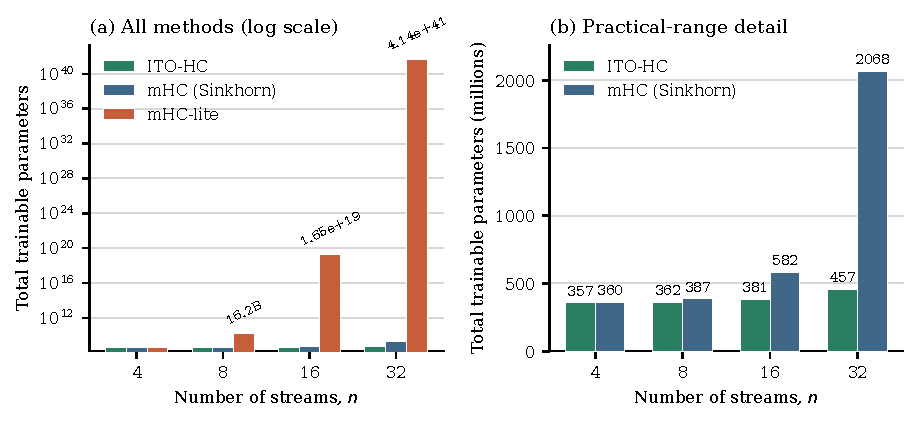
\includegraphics[width=0.96\linewidth]{figures/large_model_parameter_scaling.pdf}
\caption{Total trainable parameters for the 24-layer, $d=1024$ large model. Each Transformer block contains two hyper-connections. Panel (a) uses a logarithmic axis to include the factorial mHC-lite parameterization; labels above its $n\geq8$ bars show absolute counts. Panel (b) enlarges the ITO-HC and mHC range; bar labels report millions of parameters. Counts include the shared $354.87$M-parameter GPT backbone and exclude non-trainable buffers.}
\label{fig:parameter-scaling}

\add{\small [[Shi-Yuk: Proposed change of Figure 1. I propose both y axes use a log scale, and that the y axis track parameters in addition to the 355M backbone. This makes it easier to compare backbone size with HC overhead, and also echos with Table 1. Please re-plot, as I do not have the actual parameter numbers; this plot is for reference only. Also consider inserting a PDF instead of a PNG for sharper rendering.]]}
\end{figure}

\subsection{Residual-mixer stability analysis}
\add{[[Shi-Yuk: Move this subsection before Section 2.1 and 2.2. Table 1 compares Sinkhorn, permutation mixtures, and Kronecker DS factors, and uses ``DS''; all of these are introduced here. You may also expand this subsection into a  related work subsection, right after introduction.]]}

\add{HC parameterizes $\Hres_l$ as a learnable static matrix, initialized to $I$, plus a dynamic term: $\tanh$ of a linear projection of the normalized stream state, scaled by a small learnable factor \citep{zhu2024hyper}.
The $\tanh$ bounds only the dynamic term; the static matrix, including its diagonal, is unconstrained.
\citet{xie2026mhc} report that this compromises the identity-mapping property and permits unbounded amplification or attenuation of the residual signal.}

mHC  \add{instead} constrains $\Hres_l$ to the \del{set} \add{Birkhoff polytope of doubly stochastic (DS) matrices,}
\begin{equation}
 \mathcal B_n=\{H\geq0:H\mathbf 1=\mathbf 1,\;\mathbf 1^\top H=\mathbf 1^\top\}.
\end{equation}
\add{mHC approximates the projection onto $\mathcal B_n$ with $20$ Sinkhorn--Knopp iterations \citep{sinkhorn1967diagonal,xie2026mhc}.
\citet{xie2026mhc} motivate the constraint by two properties: every DS matrix has spectral norm at most one, and products of DS matrices remain DS.
They also describe repeated DS mixing as ``a robust feature fusion mechanism''; the paragraph below shows that, under uniform mixing, the same repetition suppresses stream differences.}
\del{Every such matrix preserves the all-ones direction and has spectral norm at most one. Under a common mixing condition, a strictly positive matrix contracts stream-difference directions. Over depth, these contractions can drive the product toward the averaging matrix $J_n=\mathbf 1\mathbf 1^\top/n$, which motivates the stability analysis in mHC \citep{xie2026mhc}.}

mHC-lite removes \add{the} finite-iteration \del{projection} error by \del{using the Birkhoff--von Neumann theorem, which represents every doubly stochastic matrix as a convex combination of permutation matrices} \add{writing $\Hres_l$ as a convex combination of the $n!$ permutation matrices, which is exact by the Birkhoff--von Neumann theorem} \citep{birkhoff1946,yang2026mhclite}.
\add{KromHC reduces this cost with Kronecker products of smaller DS factors \citep{zhou2026kromhc}.
\citet{liu2026shc} report three limitations of the Birkhoff constraint: learned mixers collapse toward the identity, non-negativity prevents subtractive corrections, and exact parameterizations require either Sinkhorn iterations or a factorial basis.}

\del{As discussed by sHC, Birkhoff-constrained mixing is restrictive because non-negativity permits only convex combinations and therefore no direct subtractive correction \citep{liu2026shc}. mHC-lite removes Sinkhorn approximation error but retains factorial parameterization and materialization costs. ITO-HC instead preserves an explicit unit diagonal and adds bounded signed off-diagonal corrections without imposing exact double stochasticity.}

\del{An independent technical blog reports a related Qwen3-scale identity ablation that retains dynamic pre/post routers while setting $H^{\mathrm{res}}=I$ \citep{shuang2026deepseek}.}
\add{A Qwen3-scale ablation by \citet{shuang2026deepseek} sets $\Hres_l=I$ and keeps the dynamic pre/post routers; the blog calls this baseline iHC.}
We \del{treat} \add{use} this \add{report} as motivation rather than evidence\del{: it is not peer reviewed and uses a different model, data volume, and implementation}\add{, because its model, data volume, and implementation differ from ours}.
\del{Our experiments test the identity-centered hypothesis independently on GPT-2-style models and state stability claims under explicit assumptions.}
\add{ITO-HC keeps the exact unit diagonal of iHC and adds signed off-diagonal terms bounded by $\gamma_l$.
Unlike HC, it bounds the whole deviation from $I$, not only the dynamic part; unlike mHC, mHC-lite, and KromHC, it does not impose exact double stochasticity.}
\add{[[Shi-Yuk: The citation above prints the bib placeholder ``Zhihu author (2026)''. Put the blog author's real name in the .bib. If the blog itself coined ``iHC'', write ``which the author calls iHC'' instead of ``we call this baseline iHC''.]]}

\paragraph{\del{When repeated positive mixing erases stream differences.} \add{Repeated DS mixing contracts stream differences.}}
\add{[[Shi-Yuk: In this paragraph, rename $M_L$ to $G_L$ (Sec 3.2 already calls this product $G_t$, and Sec 3.1 uses $M$ for $\mathbf 1\mathbf 1^\top-I$), write $\Hres_l$ instead of $H_l$, and use the index convention of Sec 4 ($l=0,\ldots,L-1$). For page budget, keep the statement (entries at least $\varepsilon$ give $\norm{G_L-J_n}_2\leq(1-n\varepsilon)^L$) and move the invariant-subspace steps to the appendix.]]}
Let $G_L=\Hres_{L-1}\cdots\Hres_0$ and $J_n=\mathbf 1\mathbf 1^\top/n$, where $\Hres_l\in\mathcal B_n$ for $l=0,\ldots,L-1$. Every doubly stochastic matrix preserves the mean direction and the stream-difference subspace $\mathbf 1^\perp$. Define
\begin{equation}
 \rho_l=\left\|\Hres_l\big|_{\mathbf 1^\perp}\right\|_2.
 \label{eq:ds-contraction}
\end{equation}
Then $\|G_L-J_n\|_2\leq\prod_{l=0}^{L-1}\rho_l$. In particular, if every entry of every mixer is at least $\varepsilon>0$, then $\rho_l\leq1-n\varepsilon$ and
\begin{equation}
 \|G_L-J_n\|_2\leq(1-n\varepsilon)^L,\qquad
 \sigma_{\min}(G_L)\leq(1-n\varepsilon)^L\longrightarrow0.
 \label{eq:ds-smin-decay}
\end{equation}
Thus, under a common positive-mixing lower bound, the product preserves the mean direction but exponentially suppresses stream-difference directions and approaches the rank-one averaging matrix $J_n$. The invariant-subspace proof is given in Appendix~\ref{app:ds-proof}. Double stochasticity alone is not enough: a sequence of identity or permutation matrices exhibits no such decay. 
\add{The bound describes how the residual path transports an earlier contribution. Each branch still writes new stream differences through $\Hpost_l$.}
\del{Strict positivity often induces this contraction, but a uniform bound requires a common mixing condition, such as a lower bound on positive entries; double stochasticity alone does not imply it.}
Finite Sinkhorn--Knopp iterations introduce a separate issue: the output need not be exactly doubly stochastic, so neither the invariant-subspace argument nor the contraction bound applies exactly\add{~\citep{yang2026mhclite}}.

\add{[[Shi-Yuk: sHC reports that learned Birkhoff mixers collapse around the identity, which would make $\rho_l$ close to $1$ and this contraction weak in practice. Add a numerical measurement: report $\rho_l$ per layer, and its product, for mHC and our ITO-HC (M, $n=4$, or scale-up if computation allows)), so the argument is also backed by numerical measurement. Report in somewhere in Section 3, 4 or 5.]]}

\add{[[Shi-Yuk: I think mHC exponentiates the logits before Sinkhorn, every mHC mixer is strictly positive. Add one sentence highlighting this property, as this gives $\rho_l<1$ strictly at every mHC layer.]]}

In the standard mHC construction, exponentiating finite logits before Sinkhorn produces strictly positive entries before normalization; hence each realized mHC mixer is strictly positive and has $\rho_l<1$ for that layer. A depth-uniform contraction rate still requires a uniform lower bound on the entries, which is why double stochasticity alone is insufficient for the bound above.



\section{ITO-HC}

\subsection{Parameterization}
Let $S_l(X_l)\in\R^{n\times n}$ denote the residual logits after the dynamic/static decomposition. Define $M=\mathbf 1\mathbf 1^\top-I$ and
\begin{equation}
 E_l=\gamma_l M\odot\tanh(S_l),\qquad \Hres_l=I+E_l.
 \label{eq:full-method}
\end{equation}
The diagonal is exactly one and $|E_{l,ij}|<\gamma_l$ for $i\ne j$. In our implementation, $\gamma_l$ is represented by an exponential log-scale, initialized to $0.05$ in the ITO-HC configuration and learned independently at each layer. The residual-logit generator can be disabled, in which case $S_l$ is static and only the pre/post routers remain dynamic.

Unlike a Sinkhorn matrix, Eq.~\ref{eq:full-method} is neither necessarily nonnegative nor doubly stochastic. Exact preservation of the mean direction would additionally require $E_l\mathbf 1=0$ and $\mathbf 1^\top E_l=0$. We use the identity-centered signed perturbation as a stability--expressivity trade-off and measure violations of these constraints rather than assuming them away.

\subsection{Layer-attention derivation}
We now derive the scalar influence of an earlier branch on a later branch input. Set $X_0=\Hpost_0y_0$ and recursively expand Eq.~\ref{eq:update}. For $i<j$,
\begin{equation}
 X_{j-1}=\sum_{i<j}\left(\prod_{k=i+1}^{j-1}\Hres_k\right)\Hpost_i y_i,
\end{equation}
and therefore
\begin{equation}
 z_j=\sum_{i<j}a_{ji}y_i,\qquad
 a_{ji}=\Hpre_j\left(\prod_{k=i+1}^{j-1}\Hres_k\right)\Hpost_i.
 \label{eq:aji}
\end{equation}
Stacking the branch outputs gives $Z=AY$. Under the source/target indexing above, $A$ is strictly lower triangular. For iHC,
\begin{equation}
 a_{ji}=\Hpre_j\Hpost_i.
 \label{eq:identity-a}
\end{equation}
Let $p_j=(\Hpre_j)^\top\in\R^n$ and $q_i=\Hpost_i\in\R^n$, and define $P=[p_1^\top;\ldots;p_T^\top]$ and $Q=[q_1^\top;\ldots;q_T^\top]$. The unmasked channel-strength matrix is
\begin{equation}
 C=PQ^\top,\qquad \operatorname{rank}(C)\le n.
 \label{eq:rank}
\end{equation}
Equation~\ref{eq:rank} characterizes the \emph{dense, unmasked scalar routing kernel}. When $n<T$, it cannot represent a target matrix whose rank exceeds $n$; the corresponding singular-value tail is the routing energy that a fixed rank-$n$ identity kernel cannot capture.

The actual causal layer matrix is instead
\begin{equation}
 A=L\odot(PQ^\top),\qquad L_{ji}=\mathbb{1}[i<j].
 \label{eq:masked}
\end{equation}
The rank bound does not generally survive the Hadamard mask:
\begin{equation}
 \operatorname{rank}\!\left(L\odot(PQ^\top)\right)\nleq n.
\end{equation}
With shifted indexing, in which target $z_j$ is paired with source $y_{j-1}$, the causal matrix is lower triangular and may have a nonzero diagonal. It can therefore be full rank even under iHC. Thus, $n<T$ restricts only the unmasked dense completion $C$; it does not prove that the causal matrix $A$, or the full nonlinear Transformer, lacks full-rank expressive power. Moreover, because $P$ and $Q$ depend dynamically on the stream state, the model represents an input-conditioned family of low-rank dense kernels rather than a single fixed matrix.

For ITO-HC, substituting Eq.~\ref{eq:full-method} into Eq.~\ref{eq:aji} yields
\begin{equation}
 a_{ji}=\Hpre_j\Hpost_i+
 \sum_{k=i+1}^{j-1}\Hpre_jE_k\Hpost_i+O(E^2).
 \label{eq:path-correction}
\end{equation}
The first term is the factorized identity kernel and the remaining terms are signed path corrections. They evolve the stream representation with depth, but Eq.~\ref{eq:path-correction} alone does \emph{not} establish a higher matrix rank. Suppose that every $\Hres_k=I+E_k$ is invertible, as guaranteed by $\norm{E_k}_2<1$, and define
\begin{equation}
 G_t=\Hres_t\Hres_{t-1}\cdots\Hres_1,
 \qquad G_0=I.
\end{equation}
Then the interval transition factorizes as
\begin{equation}
 \prod_{k=i+1}^{j-1}\Hres_k=G_{j-1}G_i^{-1},
\end{equation}
and hence
\begin{equation}
 a_{ji}
 =\underbrace{\Hpre_jG_{j-1}}_{\widehat p_j^\top}
  \underbrace{G_i^{-1}\Hpost_i}_{\widehat q_i}.
 \label{eq:gauge-factorization}
\end{equation}
Therefore the corresponding unmasked dense completion is
\begin{equation}
 C_{\mathrm{ITO\text{-}HC}}=\widehat P\widehat Q^\top,
 \qquad \operatorname{rank}(C_{\mathrm{ITO\text{-}HC}})\le n.
 \label{eq:ito-rank}
\end{equation}
For this scalar analysis, residual transitions are a depth-dependent change of stream coordinates and can be absorbed into effective read/write factors. A non-identity $\Hres$ therefore does not, by itself, give complete expressivity. Its effect is instead to transform the state before later nonlinear branches and dynamic routers are evaluated, changing activations and Jacobians while retaining an explicit identity highway.

An unconditional full-rank dense kernel for $n<T$ would require a mechanism that cannot be absorbed into one $n$-dimensional state-space factorization. Examples include a sum of independent routing kernels, pair-dependent source--target transitions, or a direct full-rank layer-routing term. ITO-HC provides no such guarantee; its practical capacity must instead be evaluated using the language-model and routing diagnostics in Section~\ref{sec:experiments}.

\subsection{Role of dynamic pre/post routing}
\label{sec:dynamic-pre-post}

The pre and post routers act on different factors of the stream--feature representation. We analyze this distinction under the identity-residual simplification $\Hres_l=I$, using the per-token state
\(X_l\in\R^{n\times C}\). Here $n$ is the number of residual streams, $C$ is the channel width, and $L$ is the number of accumulated branches. Write
\begin{equation}
 a_l(X_l)=\Hpre_l(X_l)\in\R^{1\times n},\qquad
 b_l(X_l)=\Hpost_l(X_l)\in\R^{n\times 1}.
 \label{eq:dynamic-ab}
\end{equation}
The exact branch update is
\begin{equation}
 \Phi_l(X_l)=X_l+b_l(X_l)y_l,\qquad
 y_l=f_l\!\left(a_l(X_l)X_l\right),
 \label{eq:identity-dynamic-map}
\end{equation}
where $y_l\in\R^{1\times C}$. Setting $\Hres_l=I$ preserves the nonlinear Transformer branch; it does not replace $f_l$ by an identity map.

For the feature-side interpretation, we use the local expansion
\begin{equation}
 f_l(\bar z_l+\delta z_l)=f_l(\bar z_l)+J_{f_l}(\bar z_l)\,\delta z_l+O(\|\delta z_l\|^2),
 \label{eq:local-linear-branch}
\end{equation}
when the local second derivatives are bounded. This is only a local approximation and is not needed for the rank bound below.

With iHC, the cumulative update over $L$ branches is
\begin{equation}
 X_L=X_0+\sum_{l=0}^{L-1}b_l(X_l)y_l.
 \label{eq:dynamic-sum}
\end{equation}
Define the stream-side and feature-side factors
\begin{equation}
\begin{aligned}
 B_L(X)&=\begin{bmatrix}b_0(X_0)&b_1(X_1)&\cdots&b_{L-1}(X_{L-1})\end{bmatrix}\in\R^{n\times L},\\
 Y_L(X)&=\begin{bmatrix}y_0\\y_1\\\vdots\\y_{L-1}\end{bmatrix}\in\R^{L\times C}.
\end{aligned}
 \label{eq:dynamic-by}
\end{equation}
Thus
\begin{equation}
 \begin{aligned}
 X_L-X_0&=B_L(X)Y_L(X),\\
 \operatorname{rank}(X_L-X_0)
 &\leq\min\{\operatorname{rank}(B_L(X)),\operatorname{rank}(Y_L(X))\}
 \leq\min\{n,C,L\}.
 \end{aligned}
 \label{eq:dynamic-output-rank}
\end{equation}
The last inequality is a statement about each fixed input and each token in this simplified stream--feature view. It is not a claim about the rank of the full sequence-level attention Jacobian.

\paragraph{Fixed-input matrix space.}
For a fixed input, $B_L(X)Y_L(X)$ is one matrix rather than a linear space. The relevant linear envelope is obtained by holding $B_L(X)$ fixed and allowing the branch-output coefficients to vary:
\begin{equation}
 \mathcal S_X:=\{B_L(X)Y:Y\in\R^{L\times C}\}
 =\{M\in\R^{n\times C}:\operatorname{col}(M)\subseteq U_X\},
 \qquad U_X:=\operatorname{col}(B_L(X)).
 \label{eq:fixed-input-output-space}
\end{equation}
If $r_X=\operatorname{rank}(B_L(X))$, then
\begin{equation}
 \dim\mathcal S_X=r_XC\leq LC.
 \label{eq:fixed-input-space-dim}
\end{equation}
Indeed, if $u_1,\ldots,u_{r_X}$ is a basis of $U_X$, then $\{u_i e_c^{\top}\}_{i,c}$ is a basis of $\mathcal S_X$. The actual branch outputs are constrained by $f_l$, attention, and the state recursion, so the network's reachable set is generally a subset of $\mathcal S_X$.

When $n>L$, every element of $\mathcal S_X$ has rank at most $L<n$ (and at most $\operatorname{rank}(B_L(X))$). Thus the update cannot be full row rank in the stream dimension for any individual input, even if the coefficients in $Y_L$ were unrestricted. If $C\geq n$, it is also strictly rank deficient as an $n\times C$ matrix. If $L\leq\min(n,C)$ and both factors were allowed to range freely, the largest possible envelope over all $B_L$ would be the determinantal variety
\begin{equation}
 \mathcal D_L:=\{M\in\R^{n\times C}:\operatorname{rank}(M)\leq L\},
 \qquad
 \dim\mathcal D_L=L(n+C-L).
 \label{eq:rank-variety}
\end{equation}
The actual model realizes only a constrained subset of this variety. Moreover, $\mathcal D_L$ is not a linear space; its linear span can nevertheless be all of $\R^{n\times C}$. This distinction is important when interpreting rank as an expressivity measure.

\paragraph{Static routing.}
For static pre and post routers, write $a_l(X_l)=a_l^0$ and $b_l(X_l)=b_l^0$. Then
\begin{equation}
 B_L(X)=B_L^0=\begin{bmatrix}b_0^0&\cdots&b_{L-1}^0\end{bmatrix},
 \qquad U_X=U_0:=\operatorname{col}(B_L^0),
 \label{eq:static-routing-basis}
\end{equation}
for every input. Consequently, all cumulative updates lie in the same fixed matrix space
\begin{equation}
 \mathcal S_{\mathrm{static}}=\{B_L^0Y:Y\in\R^{L\times C}\},
 \qquad
 \dim\mathcal S_{\mathrm{static}}=\operatorname{rank}(B_L^0)C\leq LC.
 \label{eq:static-output-space}
\end{equation}
The feature matrix $Y_L(X)$ is not itself fixed: nonlinear branches, attention, MLPs, and the evolving residual state can all depend on the input. The static restriction is that these input-dependent features are read and written through fixed stream-side directions. Thus the basis $\{u_i e_c^\top\}$ is fixed, while its coefficients may change with the input.

If post routing is static but pre routing is dynamic, $B_L^0$ and $\mathcal S_{\mathrm{static}}$ remain unchanged. Dynamic pre can nevertheless enlarge the set of attainable coefficient matrices $Y_L(X)$ and therefore the subset of $\mathcal S_{\mathrm{static}}$ reached by the network. It does not, by itself, create new stream-side basis directions.

\paragraph{Dynamic routing and input-conditioned spaces.}
With dynamic post routing,
\begin{equation}
 B_L(X)=\begin{bmatrix}b_0(X_0)&\cdots&b_{L-1}(X_{L-1})\end{bmatrix},
 \qquad U_X=\operatorname{col}(B_L(X)).
 \label{eq:dynamic-post-basis}
\end{equation}
The model therefore produces a family of fixed-input envelopes $\{\mathcal S_X:X\in\mathcal X\}$ rather than one common space. If $\operatorname{rank}(B_L(X))=r$ is locally constant, $U_X$ is an element of the Grassmannian $\mathrm{Gr}(r,n)$; static routing corresponds to one point in this Grassmannian, whereas dynamic post routing can trace a nontrivial input-dependent subset of it. The full Grassmannian has dimension $r(n-r)$, but the reachable subset is limited by the router parameterization and by the residual states encountered during inference.

Define the global stream span
\begin{equation}
 U_{\mathrm{global}}:=\operatorname{span}_{X\in\mathcal X}U_X,
 \qquad r_{\mathrm{global}}:=\dim U_{\mathrm{global}}\leq n.
 \label{eq:global-dynamic-stream-space}
\end{equation}
The linear span of the dynamic envelopes satisfies
\begin{equation}
 \operatorname{span}_{X\in\mathcal X}\mathcal S_X
 =U_{\mathrm{global}}\otimes\R^C,
 \qquad
 \dim\!\left(\operatorname{span}_{X}\mathcal S_X\right)=r_{\mathrm{global}}C,
 \label{eq:global-dynamic-output-space}
\end{equation}
whereas the union $\bigcup_X\mathcal S_X$ is generally not a linear space. The equality describes the coefficient-relaxed envelope; the actual outputs $\{X_L(X)-X_0(X)\}$ form a potentially smaller, nonlinear subset. In particular, dynamic post can make $r_{\mathrm{global}}$ substantially larger than $L$, and in principle $r_{\mathrm{global}}=n$, while each individual update still has rank at most $L$.

Dynamic pre routing changes the feature-side factor. With $z_l=a_l(X_l)X_l$ and a perturbation $U$,
\begin{equation}
 Dz_l[U]=a_l(X_l)U+(Da_l(X_l)[U])X_l.
 \label{eq:dynamic-read-differential}
\end{equation}
Using the local expansion in Eq.~\eqref{eq:local-linear-branch},
\begin{equation}
 \delta y_l\simeq J_{f_l}(\bar z_l)\left[a_l(\bar X_l)\delta X_l+(Da_l(\bar X_l)[\delta X_l])\bar X_l\right].
 \label{eq:dynamic-pre-linearized}
\end{equation}
The second term is absent for static pre routing. It can therefore change the attainable feature-side coefficient matrices $Y_L(X)$ even when $B_L$ is static. When post routing is also dynamic, the resulting state changes can additionally affect later columns of $B_L(X)$.

At the level of the local output geometry, the factorization gives
\begin{equation}
 D\!\left(B_LY_L\right)[U]
 =\left(DB_L[U]\right)Y_L+B_L\left(DY_L[U]\right).
 \label{eq:dynamic-factor-differential}
\end{equation}
The first term is the direct dynamic-post contribution: it can introduce stream directions outside the current $U_X$ whenever the router differential has such directions. The second term contains the dynamic-pre contribution through the branch outputs. If $B_L=B_L^0$ is static, then $DB_L=0$ and the local tangent remains in $\mathcal S_{\mathrm{static}}$; dynamic pre changes the coefficients and feature geometry inside that fixed space. At a single branch, the corresponding chain rule is
\begin{align}
 D\Phi_l(X_l)[U]
 ={}&U+(Db_l(X_l)[U])f_l(z_l) \\[-2pt]
 &+b_l(X_l)Df_l(z_l)\!\left[a_l(X_l)U+(Da_l(X_l)[U])X_l\right].
 \label{eq:dynamic-jacobian}
\end{align}
For self-attention, $Df_l$ is the Jacobian of the full token-sequence operator; it should not be identified with the per-token low-rank factorization above.

Under iHC, the cross-layer read is
\begin{equation}
 z_l=a_l(X_l)X_0+\sum_{i<l}a_l(X_l)b_i(X_i)y_i,
 \label{eq:dynamic-cross-layer}
\end{equation}
so $a_l(X_l)b_i(X_i)$ is an input-conditioned source-to-target coefficient. This shows why increasing $n$ and using dynamic routing are complementary: increasing $n$ enlarges the ambient stream space, while dynamic routing can select different low-dimensional subspaces within it.

The same distinction applies to the channel-strength factorization. The static identity analysis gives one fixed matrix $C=PQ^\top$. With dynamic routers, the relevant object is instead
\begin{equation}
 C(X)=P(X)Q(X)^\top,\qquad \operatorname{rank}(C(X))\leq n
 \quad\text{for every fixed }X.
 \label{eq:dynamic-channel-family}
\end{equation}
Thus dynamic routing supplies an input-conditioned family of low-rank matrices; it does not remove the rank bound for an individual input.

These observations establish a geometric mechanism for richer conditional representations, but not a universal full-rank or superiority theorem. The attainable $Y_L$ and $B_L$ are coupled through the state recursion; normalization and gates can suppress router variation; and the final reducer, attention coupling, and reachable state manifold determine which internal directions affect the logits. The static/dynamic ablation in Section~\ref{sec:dynamic-pre-post-ablation} should therefore be interpreted as empirical evidence for the two routing pathways, rather than as a proof that either dynamic router is mathematically indispensable.


\section{Stability analysis}

The identity-centered form permits a direct perturbation analysis. Let $\eta_l=\norm{E_l}_2$ denote the spectral size of the residual correction at layer $l$.

Because $|E_{l,ij}|<\gamma_l$ off diagonal and $E_{l,ii}=0$, a conservative bound is
\begin{equation}
 \eta_l=\norm{E_l}_2\leq\norm{E_l}_F\leq\gamma_l\sqrt{n(n-1)}.
 \label{eq:ef}
\end{equation}
Therefore,
\begin{equation}
 \norm{\Hres_l}_2\leq1+\gamma_l\sqrt{n(n-1)}.
 \label{eq:hbound}
\end{equation}
More importantly, Weyl's singular-value perturbation bound gives
\begin{equation}
 \sigma_{\min}(I+E_l)\geq1-\norm{E_l}_2=1-\eta_l.
 \label{eq:ito-layer-smin}
\end{equation}
Consequently, if $\eta_l<1$ for every layer, the multiplicativity inequality for the smallest singular value yields
\begin{equation}
 \sigma_{\min}\!\left(\prod_{l=0}^{L-1}(I+E_l)\right)
 \geq\prod_{l=0}^{L-1}(1-\eta_l)>0.
 \label{eq:ito-product-smin}
\end{equation}
If, more strongly, $\eta_l\leq\bar\eta<1$ and $\sum_l\eta_l\leq B$, then $\log(1-x)\geq-x/(1-\bar\eta)$ on $[0,\bar\eta]$ gives the depth-uniform lower bound
\begin{equation}
 \sigma_{\min}\!\left(\prod_{l=0}^{L-1}(I+E_l)\right)
 \geq \exp\!\left(-\frac{B}{1-\bar\eta}\right)>0.
 \label{eq:ito-uniform-smin}
\end{equation}
The same perturbation budget controls the largest singular value:
\begin{equation}
 \left\|\prod_{l=0}^{L-1}(I+E_l)\right\|_2
 \leq\prod_l(1+\eta_l)\leq\exp\left(\sum_l\eta_l\right).
 \label{eq:prod-bound}
\end{equation}
Equations~\ref{eq:ito-uniform-smin}--\ref{eq:prod-bound} show that, under a bounded cumulative perturbation budget, every residual-stream direction remains bounded away from zero and infinity. This differs from uniformly positive doubly stochastic mixing: ITO-HC is centered at the full-rank identity, permits signed corrections, and is not constrained to preserve the mean while contracting $\mathbf 1^\perp$. It therefore has no architectural requirement to converge to the rank-one consensus matrix $J_n$; pure identity ($E_l=0$) is the limiting case with every singular value exactly one.

This conclusion is a sufficient conditional guarantee, not an unconditional property of a unit diagonal. If $\eta_l$ stays at a fixed nonzero value as $L\to\infty$, the lower bound $\prod_l(1-\eta_l)$ can itself vanish, and specially aligned nonsymmetric perturbations can still make the product ill-conditioned. Accordingly, ITO-HC avoids the \emph{forced positive-averaging mechanism} behind Eq.~\ref{eq:ds-smin-decay}, but it must keep the learned cumulative perturbation controlled to guarantee non-vanishing singular values. From Eq.~\ref{eq:ef}, a directly checkable sufficient condition is $\gamma_l\sqrt{n(n-1)}<1$ at every layer together with a bounded sum of these quantities. This motivates monitoring both $\eta_l$, the cumulative-product singular spectrum, and the learned $\gamma_l$ during training.

\section{Experiments}
\label{sec:experiments}

We pretrain decoder-only GPT-2-style models on OpenWebText \citep{gokaslan2019openwebtext}. The repository configurations are small (6 layers, 8 heads, $d=512$), medium (12 layers, 12 heads, $d=768$), and large (24 layers, 16 heads, $d=1024$). Runs use sequence length 1024, micro-batch size 2, accumulation 128, bfloat16, AdamW (weight decay $0.1$), gradient clipping at $1.0$, and 10,000 optimizer iterations. Learning rates are $10^{-3}$, $6\times10^{-4}$, and $3\times10^{-4}$, with 200 warm-up iterations followed by cosine decay to one-tenth of the initial value.

For identity, ITO-HC, and mHC we sweep $n\in\{4,8,16,32,64\}$. Identity fixes $\Hres=I$; ITO-HC uses Eq.~\ref{eq:full-method} with $\gamma_l$ initialized to $0.05$; mHC uses its standard dynamic residual parameterization and Sinkhorn projection. We also include the single-stream residual baseline and mHC-lite at $n=4$. All multi-stream comparisons use the repository's $4$-mean reducer and repeated initial expansion. Table~\ref{tab:experiments} reports the currently available losses; missing entries remain explicit rather than being imputed.

\subsection{Why scale the number of streams?}
The original mHC and mHC-lite studies use $n=4$ for their main comparisons, while KromHC additionally tests selected larger widths \citep{xie2026mhc,yang2026mhclite,zhou2026kromhc}. Thus $n=4$ is a practical baseline, but the effect of controlled width scaling remains open.

\paragraph{Intermediate-state capacity.}
The capacity benefit of multiple streams is most transparent before the final stream reducer. Under the identity-residual abstraction used in Section~\ref{sec:dynamic-pre-post}, the cumulative branch update is
\begin{equation}
 \Delta_L(X):=X_L-X_0=B_L(X)Y_L(X),
 \qquad B_L(X)\in\R^{n\times L},\quad Y_L(X)\in\R^{L\times C}.
 \label{eq:stream-scaling-update}
\end{equation}
For a fixed input, let $U_X=\operatorname{col}(B_L(X))$ and $r_X=\operatorname{rank}(B_L(X))$. If the feature-side coefficients are relaxed to range over $Y\in\R^{L\times C}$, the corresponding linear envelope is
\begin{equation}
 \mathcal S_X=\{B_L(X)Y:Y\in\R^{L\times C}\},
 \qquad \dim\mathcal S_X=r_XC\leq\min(n,L)C.
 \label{eq:stream-scaling-space}
\end{equation}
The inequality follows because $B_L(X)$ has only $L$ columns. Thus $n$ controls the number of independent stream-side directions that can be used to store and recombine branch features, while $L$ controls the number of branch contributions available in the cumulative factorization.

The single-stream residual baseline corresponds to $n=1$. In that case $r_X\leq1$ and, whenever the update is nonzero, $\dim\mathcal S_X=C$: all branch outputs are accumulated in one residual vector. For multiple streams with sufficiently independent post factors, $r_X$ can grow to $\min(n,L)$, giving up to $\min(n,L)C$ coefficient degrees of freedom and the per-input rank bound
\begin{equation}
 \operatorname{rank}(\Delta_L(X))\leq\min(n,C,L).
 \label{eq:stream-scaling-rank}
\end{equation}
For example, two independent write directions can preserve two different branch features in two stream rows, whereas a single stream can only store their feature-space combination in one row. This is the sense in which multi-stream routing provides parallel latent memory rather than merely duplicating the final output.

The same effect appears in the layer-attention view. With $p_j=(\Hpre_j)^\top$ and $q_i=\Hpost_i$, the dense scalar routing kernel has the factorization $C=PQ^\top$ and satisfies $\operatorname{rank}(C)\leq n$ (Eq.~\ref{eq:rank}). Increasing $n$ therefore permits more independent source--target routing patterns in the unmasked completion, while dynamic pre/post routers can select different factors for different inputs. This rank statement is a capacity diagnostic rather than a theorem about the full causal Transformer, whose mask, branch Jacobians, and state recursion add further structure.

The regime $n>L$ requires a separate qualification. In that regime, $\operatorname{rank}(\Delta_L(X))\leq L<n$, so increasing $n$ beyond $L$ does not continue to raise the rank ceiling of one fixed-input cumulative update. It can nevertheless enlarge the ambient residual state, the family of input-conditioned stream subspaces $\operatorname{col}(B_L(X))$, and the state trajectories seen by later nonlinear branches. Consequently, improvements for $n>L$ should be interpreted as benefits from state-space geometry and conditional routing, not as evidence that the per-input low-rank bound has disappeared.

Finally, the $n$-stream advantage is not contradicted by the final reducer. If the output head receives $r^\top X_L$ for a fixed reducer vector $r$, then the final merged update is a $1\times C$ vector. The relevant capacity gain occurs before this merge: subsequent attention and MLP branches can read stream differences through $\Hpre_l$, transform them nonlinearly, and write new combinations through $\Hpost_l$. A reducer that is applied only after all branches therefore preserves the usefulness of intermediate stream separation, whereas merging after every branch would largely remove it. The normalized $4$-mean used below controls output amplitude across widths; it does not remove the intermediate-state routing degrees of freedom.

There is also an output-scale issue when comparing stream widths. The original mHC paper specifies the per-layer pre/post/residual hyper-connection maps, but does not explicitly specify how the final $n$ streams are merged before the language-model head. In contrast, the mHC-lite implementation used for comparison merges the streams by summation (``sum-up''),
\begin{equation}
 x_{\mathrm{out}}=\sum_{s=1}^{n}x_s,
 \label{eq:sum-reducer}
\end{equation}
which we refer to as the sum-up reducer. The repository's generic reducer also defaults to this unnormalized sum. If the stream states have comparable scale and weakly correlated signs, the norm of this sum can grow with $n$ (in the worst aligned case linearly in $n$). This creates a confounding amplitude change when $n$ is increased: a lower loss or an unstable run could reflect output rescaling rather than increased routing capacity. We therefore use the normalized reducer as follows:
\begin{equation}
 x_{\mathrm{out}}=\frac{4}{n}\sum_{s=1}^{n}x_s,
 \label{eq:four-mean-reducer}
\end{equation}
 The factor $4$ gives the $n=4$ setting the same gain as the historical sum baseline, while preventing the output gain from growing with $n$. We apply this convention to identity, ITO-HC, and the mHC stream-width sweep; the single-stream residual baseline uses its ordinary identity output.

The normalized comparison separates routing capacity from output-scale effects. Increasing $n$ enlarges the routing state, while the $4$-mean merge prevents automatic output amplification. Identity and ITO-HC add $O(dn^2)$ router parameters per hyper-connection; fully dynamic mHC adds an $O(dn^3)$ residual generator.

\subsection{Ablating dynamic pre/post routing}
\label{sec:dynamic-pre-post-ablation}
\add{[[Shi-Yuk: This section may go to the Appendix.]]}
The small-model static/dynamic ablations and the wide static-routing stress tests are reported in Appendix~\ref{app:dynamic-pre-post-ablation}. They are diagnostic comparisons rather than parameter- or memory-matched scaling experiments.

\begin{table}[t]
\caption{Repository model configurations. The labels S/M/L refer to the configurations used in this paper and are not the vanilla nanoGPT/GPT-2 model-type names. \add{[[Shi-Yuk: You may need to add a table documenting model architecture (layer, width, number of head, total params, etc., and make explicit that the size label conventions are different to the ones in vanilla nanoGPT (GPT-2).]]}}
\label{tab:model-config}
\begin{center}
\small
\begin{tabular}{lrrrr}
\toprule
Configuration & Layers & Heads & Width $d$ & Backbone parameters \\
\midrule
S & 6 & 8 & 512 & 45.20M \\
M & 12 & 12 & 768 & 124.48M \\
L & 24 & 16 & 1024 & 354.87M \\
\bottomrule
\end{tabular}
\end{center}
\end{table}

\begin{table}[t]
\caption{Available last-iteration OpenWebText losses after 10,000 iterations; lower is better. ``--'' denotes an unreported value. ITO-HC is lower than identity at every listed large-model width. \add{[[Shi-Yuk: Those loss numbers marked with asterisk (*) are identical up to all decimals. Copy-paste typo? Double check all numbers.]]}
\label{tab:experiments}
\begin{center}
{\setlength{\tabcolsep}{2pt}
\renewcommand{\arraystretch}{0.68}
\footnotesize
\add{[[Shi-Yuk: use at most footnotesize. Avoid using scriptsize for readability.]]}
\begin{tabular}{l c cc cc cc}
\toprule
Dataset & & \multicolumn{6}{c}{\texttt{OpenWebText}}\\
\cmidrule(lr){3-8}
Method & Streams $n$ & \multicolumn{2}{c}{\textsf{S}} & \multicolumn{2}{c}{\textsf{M}} & \multicolumn{2}{c}{\textsf{L}}\\
\cmidrule(lr){3-4}\cmidrule(lr){5-6}\cmidrule(lr){7-8}
& & Train & Val & Train & Val & Train & Val\\
\midrule
\multirow{5}{*}{\del{Identity}\add{iHC}}
 & 4  & 3.4270 & 3.3833 & 3.1648583 & 3.1348 & 3.0473 & 3.0842\\
 & 8  & 3.3822 & 3.3755 & 3.1501 & 3.1216 & 3.0493 & 3.0861\\
 & 16 & 3.3992 & 3.3753 & 3.1414 & 3.1128 & 3.0344 & 3.0712\\
 & 32 & 3.4200 & 3.3754 & 3.1355 & 3.1085 & 3.0290 & 3.0635\\
 & 64 & 3.3757 & 3.3607 & 3.1296 & 3.1017 & 3.0265 & 3.0606\\
\midrule
\multirow{5}{*}{ITO-HC}
 & 4  & 3.3933 & 3.3765 & 3.1589 & 3.1293 & 3.0461 & 3.081\\
 & 8  & 3.3699 & 3.3659 & 3.1487 & 3.1190 & 3.0463 & 3.0827\\
 & 16 & 3.3855 & 3.3684 & 3.1361 & 3.1085 & 3.0288 & 3.0657\\
 & 32 & 3.3774 & 3.3612 & 3.1234 & 3.0982 & 3.0187 & 3.0559\\
 & 64 & 3.3711 & 3.3573 & 3.1147 & 3.0884 & 2.9926 & 3.0310\\
\midrule
mHC & 4  & 3.3964 & 3.3817 & 3.1554024 & 3.1472 & 3.0562 & 3.0916\\
mHC-lite & 4 & 3.3931 & 3.3776 & 3.1623828 & 3.1338809 & 3.0553 & 3.0898\\
Residual & 1 & 3.4177 & 3.4598 & 3.2086 & 3.2240 & 3.0934 & 3.1277\\
\bottomrule
\end{tabular}}
\end{center}
\end{table}

The available large-model sweep shows ITO-HC improving over identity by $0.0032$, $0.0034$, $0.0056$, $0.0076$, and $0.0296$ at $n=4,8,16,32,64$; these are single-run values.

\section{Discussion and limitations}

The rank bound in Eq.~\ref{eq:rank} describes a dense scalar routing kernel, not the full Transformer. The causal mask, input-dependent routers, and branch Jacobians can all produce behavior outside that fixed factorization.

ITO-HC does not impose exact double stochasticity: its stability guarantee is conditional on accumulated perturbation norms, and signed corrections may change the stream mean. The current study is limited to OpenWebText and GPT-2-style sizes; larger-scale training and downstream transfer remain open. Routing diagnostics should therefore accompany final loss comparisons.

\section{Conclusion}

We introduced ITO-HC, an identity-centered residual mixer for multi-stream Hyper-Connections. It keeps an exact self highway, bounds signed cross-stream corrections, and preserves nonlinear branches and dynamic pre/post routing. The layer-attention analysis identifies the rank-$n$ dense kernel of iHC, while the stability analysis gives conditional bounds for ITO-HC. Experiments compare this stability--capacity trade-off with mHC and mHC-lite.

\appendix
\section{Additional derivations and ablations}

\subsection{Parameter-count derivations}
\label{app:parameter-counts}
With one fraction and one input view, the exact trainable-parameter count of the main ITO-HC configuration is
\begin{equation}
 N_{\mathrm{ITO\text{-}HC}}=2dn^2+dn+n^2+2n+3=O(dn^2),
 \label{eq:ito-param-count}
\end{equation}
where $2dn^2$ is the dynamic pre/post-router cost, $dn$ is the RMSNorm scale, $n^2$ is the static residual-logit matrix, and the remaining terms are static pre/post logits and scalar gates. The count assumes a trainable $\gamma_l$ and excludes the intentionally frozen dynamic-residual scale. The dynamic $\Hres$ generator is disabled in the main ITO-HC configuration. A minimal pure-identity implementation has the same router cost but can omit the residual-logit matrix.

For comparison, the corresponding counts for the standard parameterizations are
\begin{align}
 N_{\mathrm{mHC}} &= dn^3+(2d+1)n^2+dn+2n+3,\\
 N_{\mathrm{mHC\text{-}lite}} &= (dn+1)n!+2dn^2+dn+2n+3,\\
 N_{\mathrm{KromHC}} &= 2dn^2+dn+(dn+1)\prod_{r=1}^{K}i_r!+2n+3,
 \label{eq:prior-counts}
\end{align}
where $n=\prod_{r=1}^{K}i_r$ for KromHC. For binary modes, $\prod_r i_r!=n$; this simplification does not hold for arbitrary factors. Counts are per hyper-connection, so a depth-$L$ Transformer with two branches per block multiplies them by $2L$.

\subsection{Proof of the doubly stochastic contraction bound}
\label{app:ds-proof}
Let $\mathcal B_n$ denote the set of doubly stochastic matrices, $J_n=\mathbf 1\mathbf 1^\top/n$, and $V=\mathbf 1^\perp$. If $H\in\mathcal B_n$, then $H\mathbf 1=\mathbf 1$ and $\mathbf 1^\top H=\mathbf 1^\top$, so both $\operatorname{span}\{\mathbf 1\}$ and $V$ are invariant. In the orthogonal decomposition $\mathbb R^n=\operatorname{span}\{\mathbf 1\}\oplus V$, $H$ acts as the identity on the first summand and as $H|_V$ on the second. For $G_L=\Hres_{L-1}\cdots\Hres_0$, this gives
\begin{equation}
 G_L-J_n=\left.G_L\right|_V\oplus 0,
 \qquad
 \|G_L-J_n\|_2\leq\prod_{l=0}^{L-1}\rho_l,
 \quad \rho_l=\|\Hres_l|_V\|_2.
\end{equation}
If every entry of $\Hres_l$ is at least $\varepsilon>0$, with $n\varepsilon<1$, then
\begin{equation}
 K_l=\frac{\Hres_l-\varepsilon\mathbf 1\mathbf 1^\top}{1-n\varepsilon}
\end{equation}
is doubly stochastic. Since $\mathbf 1\mathbf 1^\top$ vanishes on $V$ and every doubly stochastic matrix has spectral norm at most one, $\rho_l=(1-n\varepsilon)\|K_l|_V\|_2\leq1-n\varepsilon$. This proves the uniform bound in Eq.~\ref{eq:ds-smin-decay}. Strict positivity without a common lower bound implies only $\rho_l<1$ separately at each layer; it does not provide a depth-independent contraction rate.

\subsection{Static/dynamic pre/post routing ablations}
\label{app:dynamic-pre-post-ablation}
\add{[[Shi-Yuk: This section may go to the Appendix.]]}
The four-way small-model ablation at $n=4$ compares dynamic/dynamic, static/static, static/dynamic, and dynamic/static routing, where the first entry denotes $\Hpre$ and the second denotes $\Hpost$. Static logits remain trainable; only the corresponding state-dependent generator is removed. Other training settings are fixed. The completed ITO-HC static/static, static/dynamic, and dynamic/static runs are reported alongside the identity ablation; the standalone ITO-HC dynamic/dynamic run remains reported in the main sweep.

The $n=70$ static run is a wider comparison, not a parameter- or memory-matched comparison: its measured throughput is $4.61\times10^5$ tokens/s versus $4.85\times10^5$ for dynamic identity at $n=4$. The $n=1024$ run is an extreme width-stress test for whether input-independent state can compensate for missing dynamic directions; it is not an equal-resource comparison. Its results should be read as small-model diagnostics rather than as a general scaling law.

\begin{table}[t]
\caption{Small-model ablation of dynamic pre/post routing for identity and ITO-HC. ``Pre/post'' specifies whether each router is dynamic or static; ``--'' marks an experiment that has not yet been run or reported. The $n=1024$ row is a width stress test.\add{[[Shi-Yuk: This table may go to the Appendix.]]}}
\label{tab:dynamic-pre-post-ablation}
\begin{center}
{\setlength{\tabcolsep}{3pt}
\renewcommand{\arraystretch}{0.9}
\small
\begin{tabular}{l c c c c}
\toprule
Configuration & Streams $n$ & Pre/post & Final train loss & Final val loss \\
\midrule \add{\multirow{6}{*}{iHC}}
 & 4 & dynamic/dynamic & 3.4270 & 3.3833 \\
 & 4 & static/static & 3.4289 & 3.4150 \\
 & 4 & static/dynamic & 3.4110 & 3.3927 \\
 & 4 & dynamic/static & 3.4185 & 3.4010 \\
 & 70 & static/static & 3.4303 & 3.4136 \\
 & 1024 & static/static & 3.4345 & 3.4168 \\
\midrule
\multirow{4}{*}{ITO-HC}
 & 4 & dynamic/dynamic & 3.3933 & 3.3765 \\
 & 4 & static/static & 3.4263 & 3.4094 \\
 & 4 & static/dynamic & 3.4043 & 3.3875 \\
 & 4 & dynamic/static & 3.4084 & 3.3925 \\
\bottomrule
\end{tabular}}
\end{center}
\end{table}

\add{[[Shi-Yuk: The bib style lowercases titles, so the references print "mhc", "kromhc", "birkhoff", etc. In the .bib, wrap every word whose capitals must be kept in braces, e.g. title={\{mHC\}: Manifold-Constrained Hyper-Connections}. Affected entries: xie2026mhc, yang2026mhclite, zhou2026kromhc, liu2026shc, shuang2026deepseek, gokaslan2019openwebtext. I have fixed some of them, check the remaining.]]}
\bibliographystyle{iclr2027_conference}
\bibliography{identity_tanh_offdiag_iclr2027}

\end{document}
